\documentclass[]{article}
\usepackage{lmodern}
\usepackage{amssymb,amsmath}
\usepackage{ifxetex,ifluatex}
\usepackage{fixltx2e} % provides \textsubscript
\ifnum 0\ifxetex 1\fi\ifluatex 1\fi=0 % if pdftex
  \usepackage[T1]{fontenc}
  \usepackage[utf8]{inputenc}
\else % if luatex or xelatex
  \ifxetex
    \usepackage{mathspec}
  \else
    \usepackage{fontspec}
  \fi
  \defaultfontfeatures{Ligatures=TeX,Scale=MatchLowercase}
\fi
% use upquote if available, for straight quotes in verbatim environments
\IfFileExists{upquote.sty}{\usepackage{upquote}}{}
% use microtype if available
\IfFileExists{microtype.sty}{%
\usepackage[]{microtype}
\UseMicrotypeSet[protrusion]{basicmath} % disable protrusion for tt fonts
}{}
\PassOptionsToPackage{hyphens}{url} % url is loaded by hyperref
\usepackage[unicode=true]{hyperref}
\hypersetup{
            pdftitle={Applying the ΔTraitSDM to a multi-site provenance trial of native Scots pine (Pinus sylvestris)},
            pdfborder={0 0 0},
            breaklinks=true}
\urlstyle{same}  % don't use monospace font for urls
\usepackage[margin=1in]{geometry}
\usepackage{color}
\usepackage{fancyvrb}
\newcommand{\VerbBar}{|}
\newcommand{\VERB}{\Verb[commandchars=\\\{\}]}
\DefineVerbatimEnvironment{Highlighting}{Verbatim}{commandchars=\\\{\}}
% Add ',fontsize=\small' for more characters per line
\usepackage{framed}
\definecolor{shadecolor}{RGB}{248,248,248}
\newenvironment{Shaded}{\begin{snugshade}}{\end{snugshade}}
\newcommand{\KeywordTok}[1]{\textcolor[rgb]{0.13,0.29,0.53}{\textbf{#1}}}
\newcommand{\DataTypeTok}[1]{\textcolor[rgb]{0.13,0.29,0.53}{#1}}
\newcommand{\DecValTok}[1]{\textcolor[rgb]{0.00,0.00,0.81}{#1}}
\newcommand{\BaseNTok}[1]{\textcolor[rgb]{0.00,0.00,0.81}{#1}}
\newcommand{\FloatTok}[1]{\textcolor[rgb]{0.00,0.00,0.81}{#1}}
\newcommand{\ConstantTok}[1]{\textcolor[rgb]{0.00,0.00,0.00}{#1}}
\newcommand{\CharTok}[1]{\textcolor[rgb]{0.31,0.60,0.02}{#1}}
\newcommand{\SpecialCharTok}[1]{\textcolor[rgb]{0.00,0.00,0.00}{#1}}
\newcommand{\StringTok}[1]{\textcolor[rgb]{0.31,0.60,0.02}{#1}}
\newcommand{\VerbatimStringTok}[1]{\textcolor[rgb]{0.31,0.60,0.02}{#1}}
\newcommand{\SpecialStringTok}[1]{\textcolor[rgb]{0.31,0.60,0.02}{#1}}
\newcommand{\ImportTok}[1]{#1}
\newcommand{\CommentTok}[1]{\textcolor[rgb]{0.56,0.35,0.01}{\textit{#1}}}
\newcommand{\DocumentationTok}[1]{\textcolor[rgb]{0.56,0.35,0.01}{\textbf{\textit{#1}}}}
\newcommand{\AnnotationTok}[1]{\textcolor[rgb]{0.56,0.35,0.01}{\textbf{\textit{#1}}}}
\newcommand{\CommentVarTok}[1]{\textcolor[rgb]{0.56,0.35,0.01}{\textbf{\textit{#1}}}}
\newcommand{\OtherTok}[1]{\textcolor[rgb]{0.56,0.35,0.01}{#1}}
\newcommand{\FunctionTok}[1]{\textcolor[rgb]{0.00,0.00,0.00}{#1}}
\newcommand{\VariableTok}[1]{\textcolor[rgb]{0.00,0.00,0.00}{#1}}
\newcommand{\ControlFlowTok}[1]{\textcolor[rgb]{0.13,0.29,0.53}{\textbf{#1}}}
\newcommand{\OperatorTok}[1]{\textcolor[rgb]{0.81,0.36,0.00}{\textbf{#1}}}
\newcommand{\BuiltInTok}[1]{#1}
\newcommand{\ExtensionTok}[1]{#1}
\newcommand{\PreprocessorTok}[1]{\textcolor[rgb]{0.56,0.35,0.01}{\textit{#1}}}
\newcommand{\AttributeTok}[1]{\textcolor[rgb]{0.77,0.63,0.00}{#1}}
\newcommand{\RegionMarkerTok}[1]{#1}
\newcommand{\InformationTok}[1]{\textcolor[rgb]{0.56,0.35,0.01}{\textbf{\textit{#1}}}}
\newcommand{\WarningTok}[1]{\textcolor[rgb]{0.56,0.35,0.01}{\textbf{\textit{#1}}}}
\newcommand{\AlertTok}[1]{\textcolor[rgb]{0.94,0.16,0.16}{#1}}
\newcommand{\ErrorTok}[1]{\textcolor[rgb]{0.64,0.00,0.00}{\textbf{#1}}}
\newcommand{\NormalTok}[1]{#1}
\usepackage{graphicx,grffile}
\makeatletter
\def\maxwidth{\ifdim\Gin@nat@width>\linewidth\linewidth\else\Gin@nat@width\fi}
\def\maxheight{\ifdim\Gin@nat@height>\textheight\textheight\else\Gin@nat@height\fi}
\makeatother
% Scale images if necessary, so that they will not overflow the page
% margins by default, and it is still possible to overwrite the defaults
% using explicit options in \includegraphics[width, height, ...]{}
\setkeys{Gin}{width=\maxwidth,height=\maxheight,keepaspectratio}
\IfFileExists{parskip.sty}{%
\usepackage{parskip}
}{% else
\setlength{\parindent}{0pt}
\setlength{\parskip}{6pt plus 2pt minus 1pt}
}
\setlength{\emergencystretch}{3em}  % prevent overfull lines
\providecommand{\tightlist}{%
  \setlength{\itemsep}{0pt}\setlength{\parskip}{0pt}}
\setcounter{secnumdepth}{0}
% Redefines (sub)paragraphs to behave more like sections
\ifx\paragraph\undefined\else
\let\oldparagraph\paragraph
\renewcommand{\paragraph}[1]{\oldparagraph{#1}\mbox{}}
\fi
\ifx\subparagraph\undefined\else
\let\oldsubparagraph\subparagraph
\renewcommand{\subparagraph}[1]{\oldsubparagraph{#1}\mbox{}}
\fi

% set default figure placement to htbp
\makeatletter
\def\fps@figure{htbp}
\makeatother

\usepackage{booktabs}
\usepackage{longtable}
\usepackage{array}
\usepackage{multirow}
\usepackage{wrapfig}
\usepackage{float}
\usepackage{colortbl}
\usepackage{pdflscape}
\usepackage{tabu}
\usepackage{threeparttable}
\usepackage{threeparttablex}
\usepackage[normalem]{ulem}
\usepackage{makecell}
\usepackage{xcolor}

\title{Applying the ΔTraitSDM to a multi-site provenance trial of native Scots
pine (\emph{Pinus sylvestris})}
\author{}
\date{\vspace{-2.5em}}

\begin{document}
\maketitle

This file documents the process of finding the most important climate
variables which may be influencing native Scots pine height across
Scotland. It shows the testing of a number of mixed-effects models,
their comparison, and their implementation within a ΔTraitSDM framework
to predict current and future distribution of the trait of interest.

\section{Climate variables driving
height}\label{climate-variables-driving-height}

A number of strategies have been applied to explore the data and try to
uncover the climate variables which may be explanatory for height. The
factors driving height may be: \emph{degree days below 18},
\emph{precipitation as snow}, \emph{temperature extremes} (warmest and
coldest month temperatures, degree days below 0), \emph{frost free
period} and when this begins/ends, and temperature difference between
coldest and warmest temperatures (\emph{continentality}).

The data is nested Trial/Block/Provenance. Figure @ref(fig:boxplot)
illustrates that there is variation in height between trials, and also
within trials according to provenance. So there is value in fitting a
mixed-effects model to explore height, with the random effects structure
taking account of the different trials and provenances.

\begin{figure}
\centering
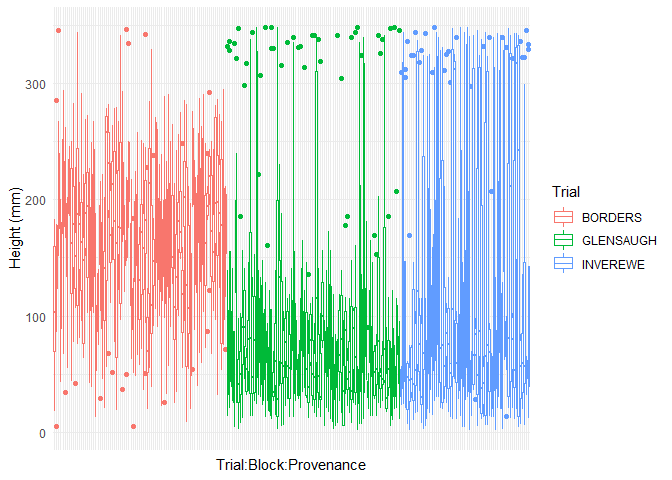
\includegraphics{scotsPine_deltaTraitSDM_files/figure-latex/boxplot-1.pdf}
\caption{Boxplot showing the variation in height at each trial site,
split by block and provenance}
\end{figure}

\section{Initial models}\label{initial-models}

A number of models combining the potentially important variables
highlighted above have been produced. These were compared via a number
of indices (Table @ref(tab:model-performance)).

\subsection{Compare model performance}\label{compare-model-performance}

\begin{table}[!h]

\caption{\label{tab:model-performance}Comparison of model indices}
\centering
\fontsize{9}{11}\selectfont
\begin{tabular}[t]{llrrlrrrr}
\toprule
Model & Type & AIC & BIC & R2\_conditional & R2\_marginal & RMSE & BF & Performance\_Score\\
\midrule
dredge3 & lmerMod & 4648.323 & 4703.234 & NA & 0.1810385 & 0.8724984 & Inf & 0.9996301\\
dredge2 & lmerMod & 4651.820 & 4706.731 & NA & 0.1810385 & 0.8724984 & Inf & 0.9995247\\
whittet.mod3 & lmerMod & 4668.797 & 4723.708 & NA & 0.1731523 & 0.8743285 & Inf & 0.9870479\\
pair.mod2 & lmerMod & 4659.232 & 4703.161 & NA & 0.1715617 & 0.8744134 & Inf & 0.9850894\\
diff.mod3 & lmerMod & 4659.937 & 4703.865 & NA & 0.1712938 & 0.8741684 & Inf & 0.9846626\\
\addlinespace
diff.mod1 & lmerMod & 4664.982 & 4708.910 & NA & 0.1027848 & 0.8739460 & Inf & 0.8806154\\
diff.mod2 & lmerMod & 4662.275 & 4706.204 & NA & 0.0769831 & 0.8745669 & Inf & 0.8415662\\
pair.mod3 & lmerMod & 4658.635 & 4702.564 & NA & 0.0598707 & 0.8757437 & Inf & 0.8157212\\
pca.mod1 & lmerMod & 4644.254 & 4688.183 & NA & 0.0572882 & 0.8728196 & Inf & 0.8122467\\
dredge1 & lmerMod & 4651.800 & 4695.729 & NA & 0.0566682 & 0.8731068 & Inf & 0.8110781\\
\addlinespace
pca.mod2 & lmerMod & 4657.633 & 4701.561 & NA & 0.0502257 & 0.8760696 & Inf & 0.8011237\\
whittet.mod2 & lmerMod & 4656.787 & 4700.715 & NA & 0.0437996 & 0.8758730 & Inf & 0.7914043\\
pca.mod3 & lmerMod & 4656.905 & 4700.834 & NA & 0.0437377 & 0.8758994 & Inf & 0.7913068\\
whittet.mod1 & lmerMod & 4641.582 & 4685.511 & NA & 0.0161882 & 0.8720915 & Inf & 0.7500000\\
pair.mod1 & lmerMod & 21225.969 & 21269.897 & NA & 0.1072019 & 89.3598514 & 1 & 0.1380247\\
\bottomrule
\end{tabular}
\end{table}

\subsection{Cross-validation}\label{cross-validation}

Using the five `best' models from the comparisons above,
cross-validation was carried out.

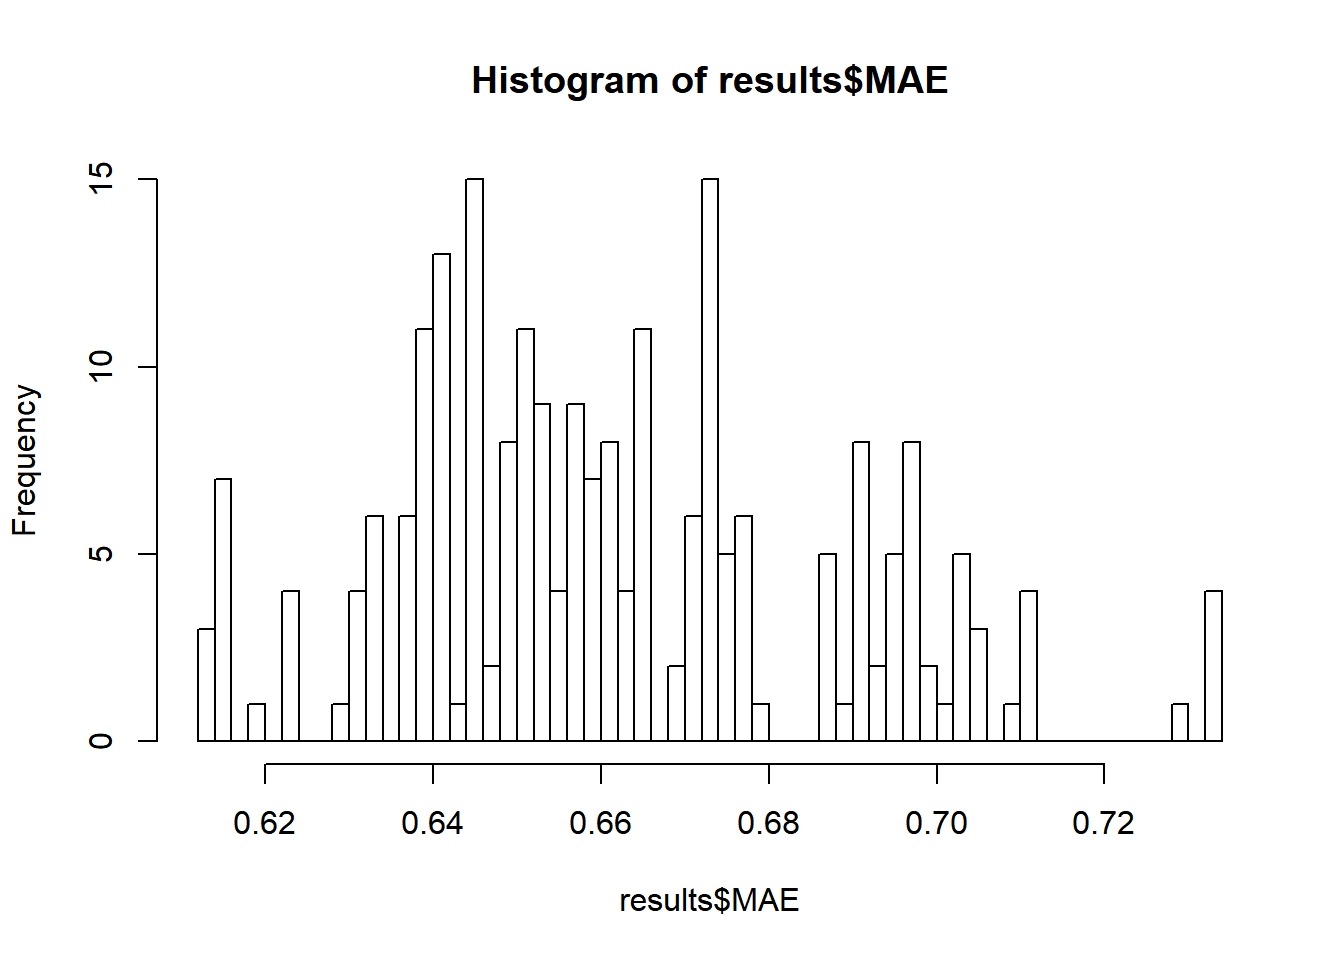
\includegraphics{scotsPine_deltaTraitSDM_files/figure-latex/cv-results-1.pdf}
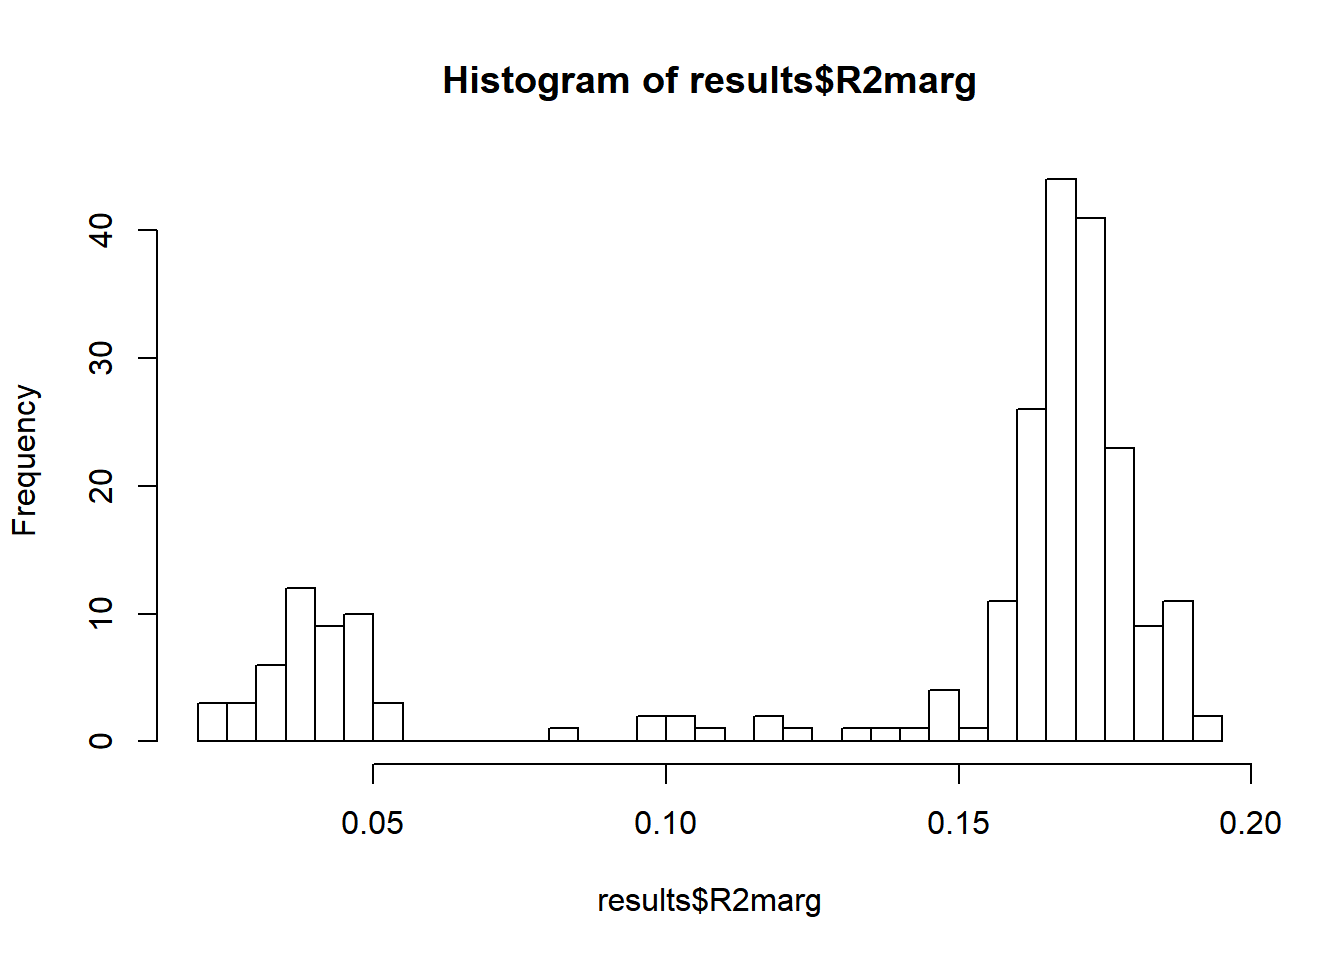
\includegraphics{scotsPine_deltaTraitSDM_files/figure-latex/cv-results-2.pdf}

The results of the cross validation indicate that ``dredge2'' and
``dredge3'' have the highest R2 marginal. Both also showed the lowest
Mean Absolute Error (MAE). These two models were therefore taken
forwards to be tested within the ΔTraitSDM framework. The two models
took the forms:

dredge2 = Height \textasciitilde{} DD\_18\_T + NFFD\_P + PAS\_T +
DD\_18\_T x NFFD\_P + NFFD\_P x PAS\_T +
(1\textbar{}Trial/Block/Provenance)

dredge3 = Height \textasciitilde{} DD\_18\_T + NFFD\_P + TD\_T +
DD\_18\_T x NFFD\_P + NFFD\_P x TD\_T+
(1\textbar{}Trial/Block/Provenance)

Their summaries are shown below:

\begin{verbatim}
## 
## ==========================================================
##                                   Dependent variable:     
##                              -----------------------------
##                                     log(W17Height)        
## ----------------------------------------------------------
## scale(DD_18_T)                           0.054            
##                                         (0.348)           
##                                                           
## scale(NFFD_P)                           0.052*            
##                                         (0.021)           
##                                                           
## scale(PAS_T)                             0.373            
##                                         (0.387)           
##                                                           
## scale(DD_18_T):scale(NFFD_P)           0.099***           
##                                         (0.023)           
##                                                           
## scale(NFFD_P):scale(PAS_T)              -0.036            
##                                         (0.023)           
##                                                           
## Constant                               4.468***           
##                                         (0.342)           
##                                                           
## ----------------------------------------------------------
## Observations                             1792             
## Log Likelihood                         -2315.910          
## Akaike Inf. Crit.                      4651.820           
## Bayesian Inf. Crit.                    4706.731           
## ==========================================================
## Note:                        *p<0.05; **p<0.01; ***p<0.001
\end{verbatim}

The summary of dredge 2 illustrates that\ldots{}

\begin{verbatim}
## 
## ==========================================================
##                                   Dependent variable:     
##                              -----------------------------
##                                     log(W17Height)        
## ----------------------------------------------------------
## scale(DD_18_T)                          -0.620            
##                                         (0.376)           
##                                                           
## scale(NFFD_P)                           0.052*            
##                                         (0.021)           
##                                                           
## scale(TD_T)                             0.893*            
##                                         (0.388)           
##                                                           
## scale(DD_18_T):scale(NFFD_P)            0.164**           
##                                         (0.054)           
##                                                           
## scale(NFFD_P):scale(TD_T)               -0.085            
##                                         (0.054)           
##                                                           
## Constant                               4.468***           
##                                         (0.143)           
##                                                           
## ----------------------------------------------------------
## Observations                             1792             
## Log Likelihood                         -2314.162          
## Akaike Inf. Crit.                      4648.323           
## Bayesian Inf. Crit.                    4703.234           
## ==========================================================
## Note:                        *p<0.05; **p<0.01; ***p<0.001
\end{verbatim}

The summary of dredge3 illustrates that\ldots{} As degree days below 18
decrease, height decreases (not significant). As the number of
frost-free days increase, height increases slightly (significant). As
continentality increases (larger annual temperature range), height
increases (signficant).

\begin{verbatim}
## Warning in nextpar(mat, cc, i, delta, lowcut, upcut): Last two rows have
## identical or NA .zeta values: using minstep
\end{verbatim}

\begin{verbatim}
## Warning in FUN(X[[i]], ...): non-monotonic profile for .sig01
\end{verbatim}

\begin{verbatim}
## Warning in confint.thpr(pp, level = level, zeta = zeta): bad spline fit
## for .sig01: falling back to linear interpolation
\end{verbatim}

\begin{verbatim}
##                                      est         L95         U95
## Intercept                     4.46837521  4.42794918  4.50880125
## scale(DD_18_T)               -0.62000819 -0.72606249 -0.51395389
## scale(NFFD_P)                 0.05189367  0.01146323  0.09232412
## scale(TD_T)                   0.89288406  0.78683001  0.99893811
## scale(DD_18_T):scale(NFFD_P)  0.16401701  0.05794192  0.27009210
## scale(NFFD_P):scale(TD_T)    -0.08545535 -0.19152139  0.02061069
##                                                 parameter
## Intercept                                       Intercept
## scale(DD_18_T)                             scale(DD_18_T)
## scale(NFFD_P)                               scale(NFFD_P)
## scale(TD_T)                                   scale(TD_T)
## scale(DD_18_T):scale(NFFD_P) scale(DD_18_T):scale(NFFD_P)
## scale(NFFD_P):scale(TD_T)       scale(NFFD_P):scale(TD_T)
\end{verbatim}

\begin{figure}
\centering
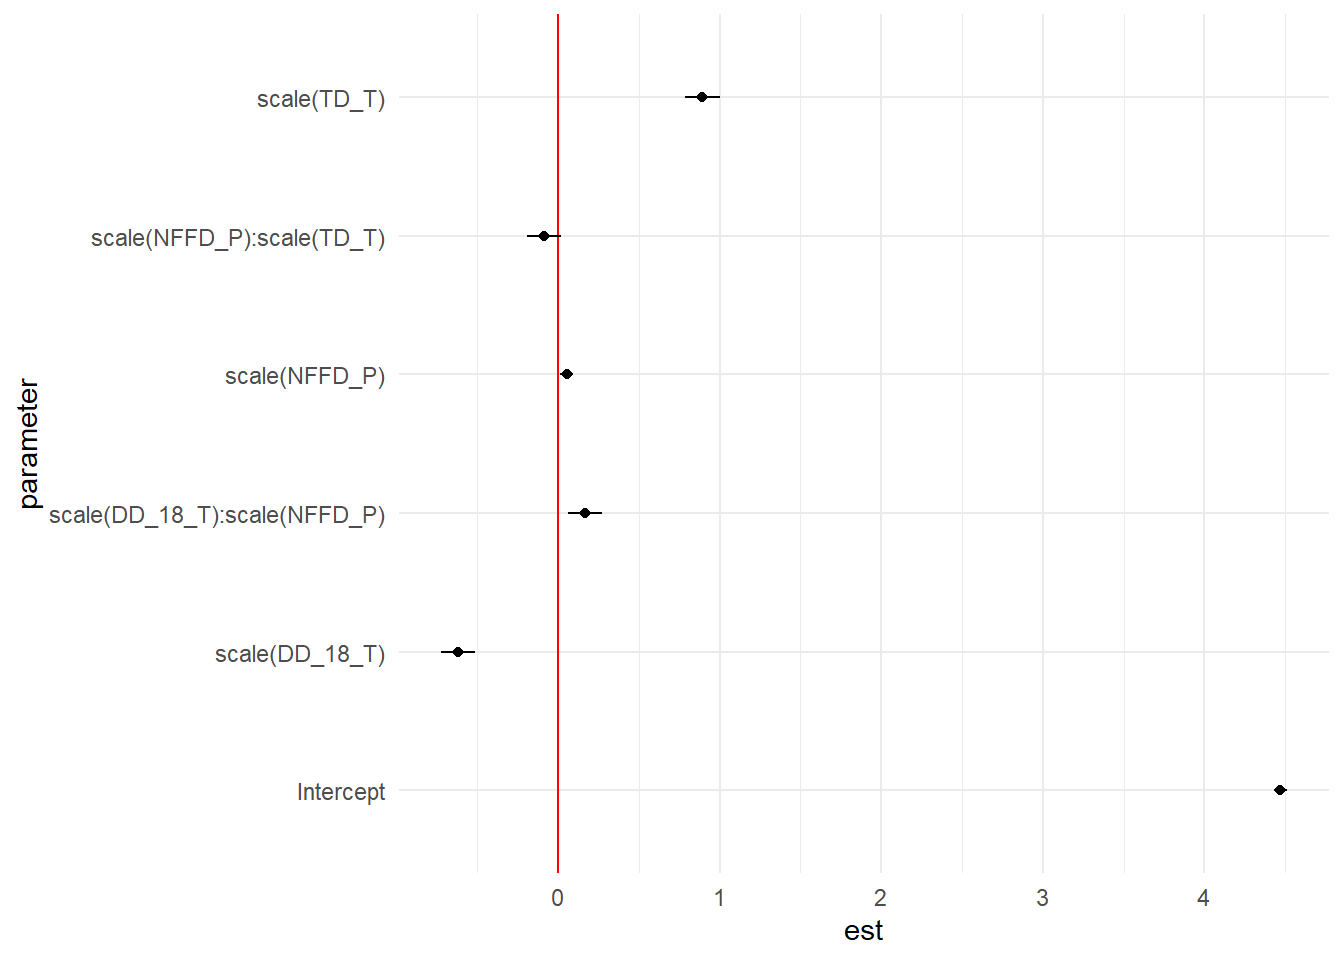
\includegraphics{scotsPine_deltaTraitSDM_files/figure-latex/visualise-fixed-1.pdf}
\caption{Visualisation of fixed effects for dredge3}
\end{figure}

\begin{Shaded}
\begin{Highlighting}[]
\CommentTok{#install.packages("devtools")}
\CommentTok{#devtools::install_github("easystats/report")}
\CommentTok{#library("report")}

\NormalTok{dredge3<-}\KeywordTok{lmer}\NormalTok{(}\KeywordTok{log}\NormalTok{(W17Height) }\OperatorTok{~}\StringTok{ }\KeywordTok{scale}\NormalTok{(DD_18_T) }\OperatorTok{+}\StringTok{ }\KeywordTok{scale}\NormalTok{(NFFD_P) }\OperatorTok{+}\StringTok{ }\KeywordTok{scale}\NormalTok{(TD_T) }\OperatorTok{+}\StringTok{ }\KeywordTok{scale}\NormalTok{(DD_18_T)}\OperatorTok{*}\KeywordTok{scale}\NormalTok{(NFFD_P) }\OperatorTok{+}\StringTok{ }\KeywordTok{scale}\NormalTok{(NFFD_P)}\OperatorTok{*}\KeywordTok{scale}\NormalTok{(TD_T)}\OperatorTok{+}\StringTok{ }\NormalTok{(}\DecValTok{1}\OperatorTok{|}\NormalTok{Trial}\OperatorTok{/}\NormalTok{Block}\OperatorTok{/}\NormalTok{Provenance),}\DataTypeTok{data =}\NormalTok{ sp.raw)}

\CommentTok{#results <- report(dredge3, ci= 95)}
\CommentTok{#table_short(results)}
\CommentTok{#text_short(results)}
\end{Highlighting}
\end{Shaded}

\section{ΔTraitSDM}\label{ux3b4traitsdm}

Several approaches were taken when applying the models within ΔTraitSDM.

Firstly, climate surfaces for the `climate normal' period (an average
taken from 1960-1990) were used to estimate distribution.

Secondly, separate climate surfaces were produced for the year when the
seed was collected for the provenance trial (2007) and the year the
seedlings were planted at the trial site (2012).

Finally, a climate surface representing possible future climate change
was used to estimate future distribution.

\subsection{Predicted distribution for current
climate}\label{predicted-distribution-for-current-climate}

Figures @ref(fig:DTSDM1) and @ref(fig:DTSDM1a) show predicted height
distribution for the current climate using the 30yr average climate
`normal' for two models.

\begin{figure}
\centering
\includegraphics{scotsPine_deltaTraitSDM_files/figure-latex/DTSDM1-1.pdf}
\caption{Height predicted using 30yr average normal climate (dredge2)}
\end{figure}

\begin{figure}
\centering
\includegraphics{scotsPine_deltaTraitSDM_files/figure-latex/DTSDM1a-1.pdf}
\caption{Height predicted using 30yr average normal climate (dredge3}
\end{figure}

Text here considering outputs from 30yr average climate data above.

\begin{figure}
\centering
\includegraphics{scotsPine_deltaTraitSDM_files/figure-latex/DTSDM2-1.pdf}
\caption{Height predicted using climate data from seed collection and
planting years}
\end{figure}

Text here considering @ref(fig:DTSDM2)\ldots{} using separate climate
rasters for seed collection year and planting year\ldots{}

These results were then masked using the current distribution of Scots
pine taken from the Native Woodland Survey Scotland\ldots{}

\begin{figure}
\centering
\includegraphics{scotsPine_deltaTraitSDM_files/figure-latex/current-dist-1.pdf}
\caption{Predicted height masked by current distribution of native Scots
pine}
\end{figure}

\subsection{Predicted distribution under future
climate}\label{predicted-distribution-under-future-climate}

Figure @ref(fig:DTSDM3) illustrates predicted height distribution for
2050 according to predicted climate for RCP 8.5.

\begin{figure}
\centering
\includegraphics{scotsPine_deltaTraitSDM_files/figure-latex/DTSDM3-1.pdf}
\caption{Tree height predicted for future climate}
\end{figure}

\section{Conclusions and next steps}\label{conclusions-and-next-steps}

\end{document}
